\newcommand{\backgroundpic}[3]{%
    \put(#1,#2){
        \parbox[b][\paperheight]{\paperwidth}{%
    		\centering
			\includegraphics[width=\paperwidth,height=\paperheight,keepaspectratio]{#3}
			\vfill
}}}

\begin{titlepage}

\AddToShipoutPicture{\backgroundpic{-4}{56.7}{framsida.pdf}}
\mbox{}
\vfill
\addtolength{\voffset}{2cm}

   



\begin{figure}[h!]
   \newcommand{\circdist}{1.2}
   \newcommand{\circrad}{2}
   \centering
   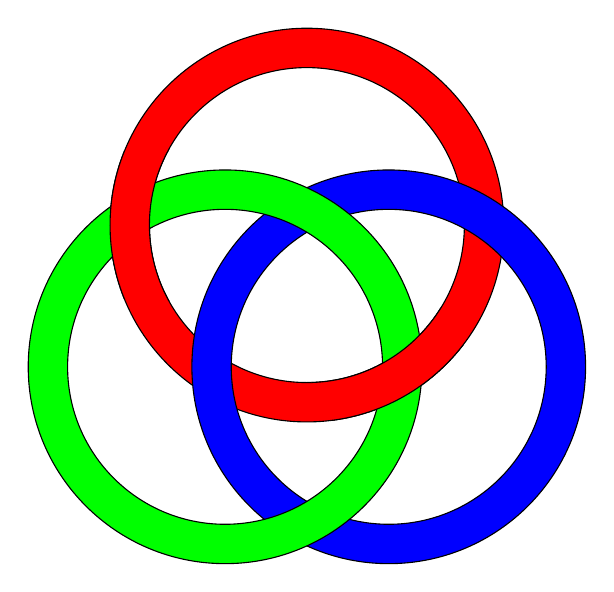
\begin{tikzpicture}[even odd rule]
     \foreach \angle/\colour in {90/red,-30/blue,210/green}
       \draw [fill=\colour] 
         (\angle:\circdist) circle (\circrad) circle (\circrad+0.5);

     \begin{scope}
     \clip (-30:\circdist) circle (1);
     \draw [fill=red] (90:\circdist) circle (\circrad) circle (\circrad+0.5);
     \end{scope}

     \clip (90:\circdist) ++ (180:\circrad) circle (1);
     \draw [fill=red] (90:\circdist) circle (\circrad) circle (\circrad+0.5);
   \end{tikzpicture}
   
\end{figure}
%\\[1 cm]



\begin{flushleft}

    {\noindent {\Huge A Study of Quantum Resonances \\ in a Complex-Momentum Basis} \\[0.5 cm]

    %{\Large Underrubrik} \\[0.5cm]

    \emph{\Large Bachelor Thesis in Physics} \\[0.5 cm]

    

	{\Large Jonathan Bengtsson, Ola Embréus, Vincent Ericsson, Pontus Granström, Nils Wireklint}\\[1 cm]

	

	{\Large Department of Fundamental Physics \\

	\textsc{Chalmers University of Technology} \\

	Göteborg, Sverige 2013 \\

    ENMX02-13-09\\

	} 

	}

\end{flushleft}



\end{titlepage}



\ClearShipoutPicture



\newpage 